\documentclass[11pt]{article}

\usepackage{sectsty}
\usepackage{graphicx}
\usepackage{forest}
\usepackage{verbatim}
\usepackage[utf8]{inputenc}
\usepackage{tikz}
\usetikzlibrary{shapes.geometric, arrows}
\usepackage[hidelinks,pdfencoding=auto]{hyperref}
\usepackage{multirow}

% Margins
\topmargin=-0.45in
\evensidemargin=0in
\oddsidemargin=0in
\textwidth=6.5in
\textheight=9.0in
\headsep=0.25in

\title{Organisation of data in standardized HDF5 Brillouin spectra containers}
\author{Pierre Bouvet}
\date{\today}

\tikzstyle{startstop} = [rectangle, rounded corners, minimum width=3cm, minimum height=1cm,text centered, draw=black, fill=red!30]
\tikzstyle{io} = [trapezium, trapezium left angle=70, trapezium right angle=110, minimum width=3cm, minimum height=1cm, text centered, draw=black, fill=blue!30]
\tikzstyle{process} = [rectangle, minimum width=3cm, minimum height=1cm, text centered, draw=black, fill=orange!30]
\tikzstyle{decision} = [diamond, minimum width=3cm, minimum height=1cm, text centered, draw=black, fill=green!30]
\tikzstyle{arrow} = [thick,->,>=stealth]

\begin{document}
\maketitle

\section{Introduction}

  The evolution of Brillouin Light Scattering (BLS) applications has lead to an increasing number of publications and research on this domain, resulting in a vast collection of data obtained with different techniques and setups by different laboratories. The evolution of this domain has reached the point where to allow it to grow outside of dedicated laboratories, a common approach to storing the data, treating them and interpreting them is needed. In an effort to facilitate this endeavour, we here propose a new structure for data organization based on the HDF5 file format.

  This document is here to explicitely define the structure of these files.

\section{Raw data}

  One of the first challenges is to allow all the users of BLS to adopt the HDF5 file format. To do so two things will be needed: a robust structure, and an interface to translate data to this structure seamlessly, robustly and reliably.

  \subsection{Concept}

    When acquiring raw spectra, we can reduce the need of the file format to two essential components:
    \begin{itemize}
      \item The informations on the data
      \item The data themselves
    \end{itemize}

    As it is possible to store information in the form of attributes inside the HDF5 file format, we hereby propose to store raw files in a HBF5 file structure as follows:

    \begin{forest}
      for tree={font=\ttfamily, grow'=0, child anchor=west, parent anchor=south, anchor=west, calign=first,
        edge path={
          \noexpand\path [draw, \forestoption{edge}]
          (!u.south west) +(7.5pt,0) |- node[fill,inner sep=1.25pt] {} (.child anchor)\forestoption{edge label};
        },
        before typesetting nodes={
          if n=1
            {insert before={[,phantom]}}
            {}
        },
        fit=band,
        before computing xy={l=15pt},
      }
      [HBH5 file
        [Attributes (type: HBF5 attributes)]
        [Data1 (type: Dataset)]
        [Data2 (type: Dataset)]
        [...]
      ]
    \end{forest} 

  \subsection{File structure}

    The limiting factor in this idea will mainly come from the name given to the dataset. Two approaches can be adopted here:
    \begin{itemize}
      \item All the data (including the data treated) will be stored in the 'Data' dataset 
      \item We separate the treated data form the 'Data' dataset
    \end{itemize} 

    Here we propose to use the second solution to distinguish the physical measures we will obtain from the values that will be derived from them. This also allows us to add in the dataset dedicated to the raw data, the calibration curves and impulse responses we might need for the treatment. As such, the structure of the HBF5 file should look like:

    \begin{forest}
      for tree={font=\ttfamily, grow'=0, child anchor=west, parent anchor=south, anchor=west, calign=first,
        edge path={
          \noexpand\path [draw, \forestoption{edge}]
          (!u.south west) +(7.5pt,0) |- node[fill,inner sep=1.25pt] {} (.child anchor)\forestoption{edge label};
        },
        before typesetting nodes={
          if n=1
            {insert before={[,phantom]}}
            {}
        },
        fit=band,
        before computing xy={l=15pt},
      }
      [HBH5 file
        [Attributes (type: HBF5 attributes)]
        [Raw Data (type: Dataset)
        [Raw spectrum]
        [Calibration spectrum]
        [Impulse response]
        [Independent coordinates]
        [...]
        ]
        [Treated Data (type: Dataset)]
      ]
    \end{forest}

    In this software, we will only focus on the generation of HDF5 data, using callable functions which will be integrable in more developped softwares.

\section{List of attributes}

In an effort to standardize the names of the attributes inside the header of the file, we propose to rely on a fixed set of names, separated in 3 main categories:
\begin{itemize}
  \item Measure: all the parameters that are measure-dependent and that are not strictly linked to the tool used to measure the BLS spectra
  \item Spectrometer: all the parameters that are instrument-dependent. This includes all the choices made at the moment of developping the spectrometer. This separation is particularly interesting for manufacturers of standard tools as they can directly refer the model of their device here and adapt their treatments to this single parameter. 
  \item File properties: all the file-related parameters that are only linked to the numerical storage of the data.
\end{itemize}

This list is prone to evolve and we encourage everyone interested in this project to share with us the parameters they feel are needed for their particular application in order to add it to the standard. These parameters are for now the ones listed below:

\begin{tabular}{|p{3.2cm} p{3cm}||p{2cm}|p{3cm}|p{1.8cm}|p{0.5cm}|}
  \hline
  Category & Parameter name & Parameter Unit or Format & Parameter description & Example & V \\
  \hline
  MEASURE & Sample & text [NA] & The sample being measured & Water & 0.1 \\
  \hline
  MEASURE & Date & Year-Month-Day-Hour-Minute-Second & The time when the sample was acquired & 24-12-25-00-00-00 & 0.1\\
  \hline
  MEASURE & Exposure & float [s] & The exposure on the sample & 0.01 & 0.1 \\
  \hline
  MEASURE & Dimension & integer [NA] & The dimensions of the measure & 3 & 0.1\\
  \hline
  MEASURE & Sampling\_matrix & ($n_x,n_y,n_z$) [NA] & The number of samples per axis & (100,100,10) & 0.1\\
  \hline
  MEASURE & Sampling\_step & ($d_x,d_y,d_z$) [$\mu m$] & The step size for each axis & (10,10,100) & 0.1\\
  \hline
  \hline
  SPECTROMETER & Type & text [NA] & The type of spectrometer being used & 6-pass TFP & 0.1\\
  \hline
  SPECTROMETER & Model & text [NA] & The model of spectrometer being used & JRS-TFP2 & 0.1\\
  \hline
  SPECTROMETER & Wavelength & float [nm] & The wavelength at which the measures were made & 780 & 0.1\\
  \hline
  SPECTROMETER & Confocality & float [AU] & The size of the confocal pinhole given in Airy Units & 0.97 & 0.1\\
  \hline
  SPECTROMETER & NA\_illumination & float [NA] & The effective numerical aperture of the illumination & 0.1 & 0.1\\
  \hline
  SPECTROMETER & NA\_detection & float [NA] & The numerical aperture of the detection lens & 0.45 & 0.1\\
  \hline
  SPECTROMETER & Detector\_model & text [NA] & The manufacturer and model of the detector & Hamamatsu Orca C11440 & 0.1\\
  \hline
  SPECTROMETER & Detector\_type & text [NA] & The type of detector & CMOS & 0.1\\
  \hline
  SPECTROMETER & Filtering\_module & text [NA] & The type of filter being used & Rubidium Cell 15cm & 0.1\\
  \hline
\end{tabular}

\begin{tabular}{|p{3.2cm}p{3cm}||p{2cm}|p{3cm}|p{1.8cm}|p{0.5cm}|}
  \hline
  Category & Parameter name & Parameter Unit or Format & Parameter description & Example & V \\
  \hline
  SPECTROMETER & Illumination\_power & float [mW] & The power of the laser being used to illuminate the sample & 25 & 0.1\\
  \hline
  SPECTROMETER & Illumination\_type & text [NA] & The type of illumination being used & CW & 0.1\\
  \hline
  SPECTROMETER & Laser\_model & text [NA] & The manufacturer and model of the laser & Cobolt Flamenco & 0.1\\
  \hline
  SPECTROMETER & Laser\_drift & float [MHz/h] & The frequency drift of the laser  & 100 & 0.1\\
  \hline
  SPECTROMETER & Phonons\_measured & text [NA] & The phonons probed by the experiment & longitudinal and transverse & 0.1\\
  \hline
  SPECTROMETER & Polarization\_prob ed\_analyzed & text [NA] & The polarization probed and analyzed by the experiment & longitudinal and transverse & 0.1\\
  \hline
  SPECTROMETER & Scan\_amplitude & float [GHz] & The frequency amplitude of single-channel spectrometers (mainly TFP) & 15.02 & 0.1\\
  \hline
  SPECTROMETER & Scanning\_strategy & text [NA] & The way the scans are performed & point-scan & 0.1\\
  \hline
  SPECTROMETER & Scattering\_angles & float [degree] & The geometry of the measure & 180 & 0.1\\
  \hline
  SPECTROMETER & Spectral\_resolution & float [MHz] & The spectral resolution of the spectrometer & 15 & 0.1\\
  \hline
  SPECTROMETER & Spectrometer\_res olution & float [MHz] & The spectrometer resolution & 100 & 0.1\\
  \hline
  SPECTROMETER & x-Mechanical\_res olution & float [$\mu m$] & The mechanical resolution along the x axis & 1 & 0.1\\
  \hline
  SPECTROMETER & y-Mechanical\_res olution & float [$\mu m$] & The mechanical resolution along the y axis & 1 & 0.1\\
  \hline
  SPECTROMETER & z-Mechanical\_res olution & float [$\mu m$] & The mechanical resolution along the z axis & 1 & 0.1\\
  \hline
\end{tabular}

\begin{tabular}{|p{3.2cm}p{3cm}||p{2cm}|p{3cm}|p{1.8cm}|p{0.5cm}|}
  \hline
  Category & Parameter name & Parameter Unit or Format & Parameter description & Example & V \\
  \hline
  SPECTROMETER & x-Optical\_res olution & float [$\mu m$] & The mechanical resolution along the x axis & 10 & 0.1\\
  \hline
  SPECTROMETER & y-Optical\_res olution & float [$\mu m$] & The mechanical resolution along the y axis & 10 & 0.1\\
  \hline
  SPECTROMETER & z-Optical\_res olution & float [$\mu m$] & The mechanical resolution along the z axis & 100 & 0.1\\
  \hline
\end{tabular}


All these parameters are indicated as attributes following this nomenclature: "Category.Parameter\_name" (for example: "MEASURE.Sample").

\section{Organization of the dimensions of the raw data}

  In order to simplify the reading of the raw data by softwares, we propose to set their dimensions as follows:
  \begin{itemize}
    \item Nth dimension: spectral channels
    \item (N-1)th dimension: (if reported) z dependence
    \item (N-2)th dimension: (if reported) y dependence
    \item (N-3)th dimension: (if reported) x dependence
    \item (N-4)th dimension: (if reported) radial angular dependence
    \item (N-4)th dimension: (if reported) azimutal angular dependence
    \item (N-5)th dimension: (if reported) temperature dependence
    \item (N-6)th dimension: (if reported) concentration dependence
    \item (N-7)th dimension and further: user-specific dimensions
  \end{itemize}

\section{HDF5\_Brillouin\_creator class structure}

  \subsection{Schematical idea}

    To facilitate the creation of HDF5 files, we have developped a Python class to create HDF5 file containers. This program works as follows: \newline

    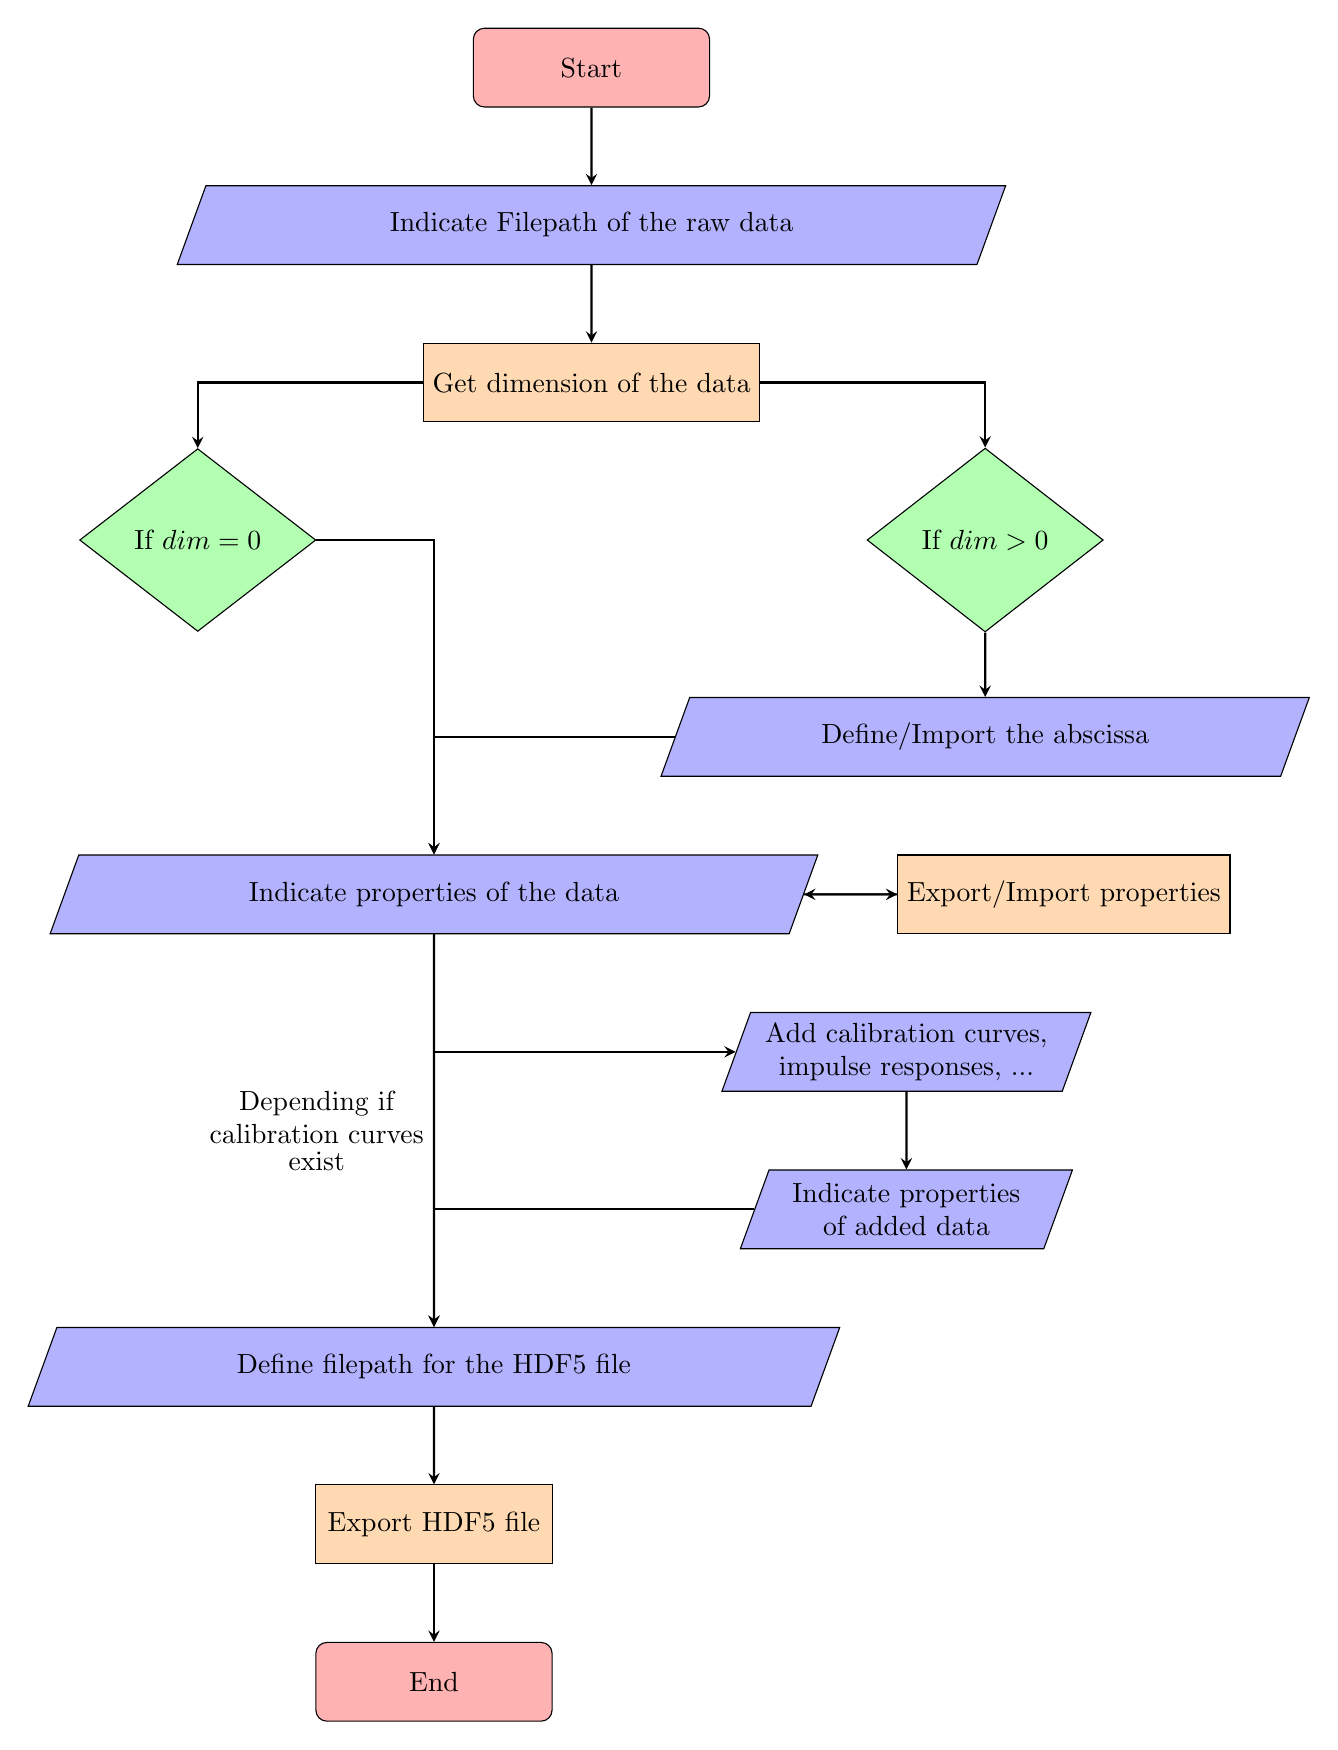
\begin{tikzpicture}[node distance=2cm]
    \node (start) [startstop] {Start};
    \node (in1) [io, below of=start] {Indicate Filepath of the raw data};
    \draw [arrow] (start) -- (in1);
    \node (pro1) [process, below of=in1] {Get dimension of the data};
    \draw [arrow] (in1) -- (pro1);
    \node (dec1) [decision, below of=pro1, xshift=-5cm] {If $dim = 0$};
    \draw [arrow] (pro1) -| (dec1);
    \node (dec2) [decision, below of=pro1, xshift=5cm] {If $dim > 0$};
    \draw [arrow] (pro1) -| (dec2);
    \node (in2) [io, below of=dec2, yshift=-0.5cm] {Define/Import the abscissa};
    \draw [arrow] (dec2) -- (in2);
    \node (in3) [io, below of=pro1, yshift=-4.5cm, xshift=-2cm] {Indicate properties of the data};
    \draw [arrow] (in2) -| (in3);
    \draw [arrow] (dec1) -| (in3);
    \node (pro2) [process, right of=in3, xshift=6cm] {Export/Import properties};
    \draw [arrow] (pro2) -- (in3);
    \draw [arrow] (in3) -- (pro2);
    \node (in4) [io, below of=in3, xshift=6cm] {\shortstack{Add calibration curves,\\impulse responses, ...}};
    \draw [arrow] (in3) |- (in4);
    \node (in4b) [io, below of=in4] {\shortstack{Indicate properties \\of added data}};
    \draw [arrow] (in4) -- (in4b);
    \node (in5) [io, below of=in4b, xshift=-6cm] {Define filepath for the HDF5 file};
    \draw [arrow] (in4b) -| (in5);
    \draw [arrow] (in3) -- node[anchor=east]{\shortstack{Depending if \\calibration curves\\exist}} (in5);
    \node (pro3) [process, below of=in5] {Export HDF5 file};
    \draw [arrow] (in5) -- (pro3);
    \node (stop) [startstop,  below of=pro3] {End};
    \draw [arrow] (pro3) -- (stop);
    \end{tikzpicture}

  \subsection{Function definitions}

  \begin{tabular}{|p{3cm}|p{5cm}|p{3cm}|p{3cm}|}
    \hline
    Function Name & Description & Arguments & Returns\\
    \hline
    self & Initiates the class & None & Nothing \\
    \hline
    open\_data & Opens a raw data file and returns the filepath & None & str (the filepath) \\
    \hline
    define\_abscissa & Defines a new abscissa axis based on minimal values, maximal values and number of values & min, max, nb\_samples & np.array (the abscissa array) \\
    \hline
    import\_abscissa & Opens an abscissa file containing the abscissa points and returns the associated array & None & np.array (the abscissa array) \\
    \hline
    properties\_data & creates a dictionnary with the given properties. All the properties are the attributes defined in section 3 of this document & **kwargs (the attributes with the key word as they will be written in the HDF5 file, for example "MEASURE.Sample") & dictionnary (the dictionnary with every attribute) \\
    \hline
    import\_properties\_data & creates a dictionnary with the given properties from a csv file. & filepath\_csv  & dictionnary (the dictionnary with every attribute) \\
    \hline
    export\_properties\_data & Asks for a csv name, and creates and saves a csv file with the properties listed in a dictionnary. & dictionnary  & filepath (the filepath of the created csv file) \\
    \hline
    open\_calibration & Asks for a calibration curve filepath and returns the calibration curve. & None & np.array \\
    \hline
    open\_IR & Asks for an Impulse response curve filepath and returns the curve. & None & np.array \\
    \hline
    save\_hdf5\_as & Asks for the filepath where to save the hdf5 file and saves it. & None & None \\
    \hline
  \end{tabular}



\end{document}
